\documentclass[a4paper]{article}

\usepackage{fullpage} % Package to use full page
\usepackage{parskip} % Package to tweak paragraph skipping
\usepackage{tikz} % Package for drawing
\usepackage{amsmath}
\usepackage{hyperref}
\usepackage{enumitem}
\title{Homework }
\author{Jeff Tilton}
\date{September, 20 2019}
\usepackage{graphicx}
\usepackage{subcaption}
\begin{document}

\maketitle

\section{K-means}

Given m = 5 data points configuration in Figure 1. Assume K = 2 and use Euclidean distance. Assuming the initialization of centroid as shown, after one iteration of k-means algorithm, answer the following questions.

\begin{enumerate}[label=(\alph*)]
\item Show the cluster assignment
\item Show the location of the new center
\item Will it terminate in one step?
\end{enumerate}

\subsection{Euclidean Distance}

\begin{enumerate}[label=(\alph*)]
\item The Cluster assignment after the first iteration is $(1,3), (2,4,5)$
\item New cluster centers are seen in figure 1 below.
\item K-means does not terminate after one step.  Centers after one step are: $(-1.5, -0.5), (1.67, 0.67)$.  After convergence: $(-1.0, -0.67), (2.5, 1.5)$
\end{enumerate}

\begin{figure}[h]
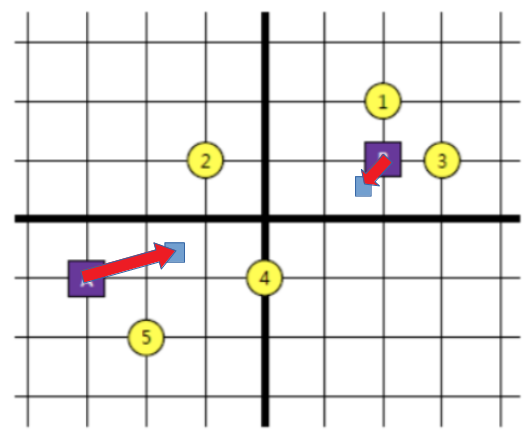
\includegraphics[width=5cm, height=5cm]{Q1_euclidean.png}
\caption{New cluster centers after one iteration of K-means using Euclidean distance}
\end{figure}



\subsection{Manhattan Distance}

\begin{enumerate}[label=(\alph*)]
\item The Cluster assignment after the first iteration is $(1,3), (2,4,5)$
\item New cluster centers are seen in figure 2 below.
\item K-means terminates after one step.  Centers after one step are: $(-1.0, -0.67), (2.5, 1.5)$.  After convergence: $(-1.0, -0.67), (2.5, 1.5)$.
\end{enumerate}

\begin{figure}[h]
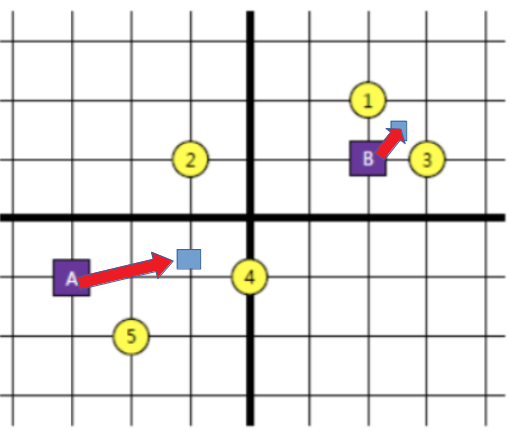
\includegraphics[width=5cm, height=5cm]{Q1_manhattan.png}
\caption{New cluster centers after one iteration of K-means using Manhattan distance}
\end{figure}


It is interesting to note the difference between the 2 measures.  Point 4 is assigned to cluster B in the Euclidean distance and pulls the cluster center towards it for the first iteration.  It then is reassigned to cluster A.  Point 4 is assigned to cluster A immediately using the Manhattan distance.  This is the reason that K-means is able to terminate after one iteration using the Manhattan distance, but multiple iterations are needed for the Euclidean distance.

\section{Spectral Clustering}

Spectral clustering goes beyond K-means, which only considers distance, and also takes the data geometry into account.  Spectral clustering uses an adjacency matrix to capture the connectedness between the data points to cluster data.  The data was clustered into 2 clusters in figure 3 below using k-nearest neighbors to create an adjacency matrix. A good way to think about this is that points are similar to each other if they can reach each other by small jumps through the data cloud.

Although nodes $(0, 0)$ and $(-1, 0)$ are closest to each other, they are in separate clusters because of the geometry of the data.  Using only K-means provided a much different result.


\begin{figure}[h]
    \centering
    \begin{subfigure}[b]{0.3\textwidth}
        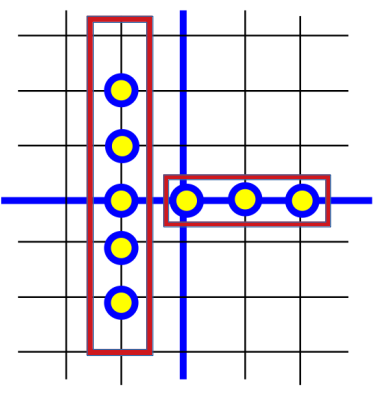
\includegraphics[width=\textwidth]{Q2_spectral.png}
        \caption{Cluster results from spectral clustering.}
        \label{spectral}
    \end{subfigure}
    \begin{subfigure}[b]{0.3\textwidth}
        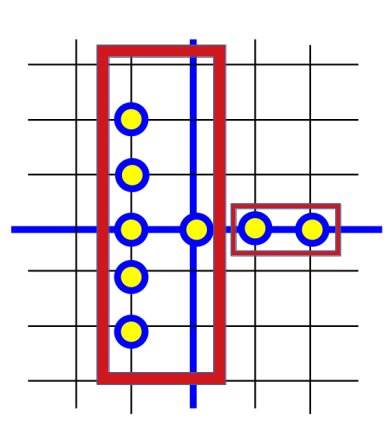
\includegraphics[width=\textwidth]{Q2_kmeans.png}
        \caption{Cluster results using K-means clustering.}
        \label{kmeans}
    \end{subfigure}

    \caption{Two different clustering algorithm results on the same dataset.  The spectral clustering used k nearest neighbors with 2 neighbors to build an adjacency matrix, then k-means on the results from eigendecomposition on the Laplacian matrix.  K-means used Euclidean distance as measure. }\label{clusterCompare}
\end{figure}

\section{Principal Component Analysis}
Suppose we have 4 points in 3-dimensional Euclidean space, namely $(4, −2, 4), (5, −3, 5),
(2, 0, 2),$ and $(3, −1, 3).$

\subsection{Find the first principal direction.}

The first principal direction is the eigenvector associated with the highest eigenvector.  THe steps listed below are how to find the $n$ principal directions of a dataset.

\begin{enumerate}
\item Standardize the data, although I found conflicting information online, a post from  Mohammad Mohammadpour Salut (@388) said to standardize the data to have a zero mean and unit variance.
\item Create the square covariance matrix.
\item Perform eigendecomposition on the covariance matrix.
\item Order the eigenvectors in descending order of their associated eigenvalues.
\item Choose the first $n$ eigenvectors as your principal components/directions.
\end{enumerate}

After performing these steps on the given data I calculated the first principal direction below. $$[ 0.57735027, -0.57735027,  0.57735027]$$.

\subsection{When we reduce the dimensionality from 3 to 1 based on the principal direction you found above, what is the reconstruction error in terms of variance?}

PCA can be thought of in 2 ways.  First, as maximizing the variance of your first $j$ components.  Or, secondly, minimizing the last $j$ components.  Eigenvalues represent the variance explained by a component, therefore the reconstruction error in terms of variance is the sum of the last 2 eigenvalues, which equals 3.02.

\newpage
\subsection{You are given the following 2-D datasets, approximately draw the first and second
principal directional on each plot.}


Optimization for PCA either maximizes the variance or minimizes the reconstruction error.  Looking at the images below, it is easy to see the first principal direction in plot a.  The variance is greatest as a negative slope, which would minimize reconstruction, much like least squares regression.  The second plot is a little harder to tell, but the first 2 principal directions form a cross with the first principal direction aligned in the vertical direction.

 

\begin{figure}[h]
    \centering
		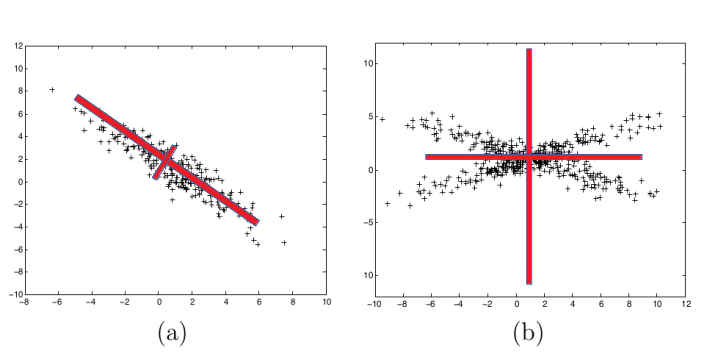
\includegraphics[width=\textwidth]{pca_clouds.png}
        \caption{The first 2 principal directions of 2 data clouds.}
\end{figure}

\bibliographystyle{plain}
\bibliography{bibliography.bib}
\end{document}